\documentclass[../src/handouts/main.tex]{subfiles}
% note that the CWD (.) above is the output directory of pdflatex
% (<repo-root-dir>/build)

% path that contains required images
\graphicspath{ {../src/handouts/figures/} }

% This document depends on introduction.tex, which provides
% fig:intro-special-functions, def:intro-equiv-relation,
% intro-equiv-relation, rem:intro-equal-sets, princ:intro-pigeonhole,
% princ:intro-induction, def:intro-tuple-ordered-pair.
% As a result, compiling only this document gives undefined references.

% prevent \recall theorems outside this section
% if this section is compiled solely
\def\sectionprefix{con}%

\begin{document}

\section{Fundamental Concepts}

% argument can be: empty or any string. Any non empty string will produce a graph with labels (people, jobs)
% ref: https://stackoverflow.com/a/2145370
\newcommand\bipartitegraphhelper[1]{
  \begin{tikzpicture}[
      point/.style = {circle, fill=black, inner sep=1mm}]
    \def \distance {1.5} %
    \foreach \x in {0,...,3} % 0 = leftmost; 3 = rightmost
    \foreach \y in {0,...,1} % 0 = top row; 1 = bottom row
    \node[point] (\y\x) at (\x * \distance, \y * - \distance) {};

    \draw (00) -- (10) -- (01) -- (11) -- (03) -- (10);
    \draw (12) -- (02) -- (13);

    % ref: https://tex.stackexchange.com/a/195498
    \ifthenelse{\isempty{#1}}%
    {}%
    {
      \node at (4 * \distance, 0) {people}
      node at (4 * \distance, - \distance) {jobs};
    }%
  \end{tikzpicture}
}%

\def \bipartitegraph{\bipartitegraphhelper{}}%

\def \bipartitegraphwithlabels {\bipartitegraphhelper{with labels}}%

\def \tripartitegraph {%
  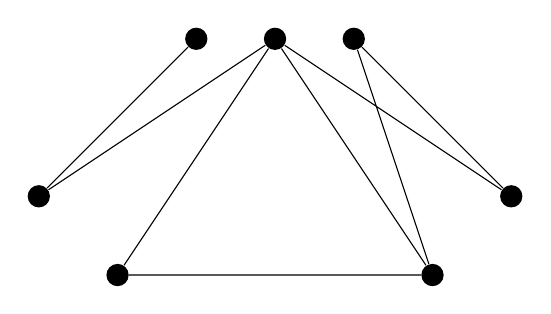
\begin{tikzpicture}[every node/.style = {circle, fill=black, inner sep=1mm}]
    \node (a1) at (-3, 1) {} % left, top
    node (a2) at (-2, 0) {} % left, bottom
    node (b1) at (-1, 3) {} % top, left
    node (b2) at (0, 3) {} % top, middle
    node (b3) at (1, 3) {} % top, right
    node (c1) at (2, 0) {} % right, bottom
    node (c2) at (3, 1) {}; % right, top
    \draw (b1) -- (a1) -- (b2) -- (a2) -- (c1) -- (b2) -- (c2) -- (b3) -- (c1);
  \end{tikzpicture}
}%

This section is the chapter one in the textbook "Introduction to Graph Theory". It covers all key concepts, keywords, definitions, theorems, etc.

\subsection{Graph}

\begin{definition}{}{con-graph}
  (1.1.2. Definition in text, modified version)
  A \textbf{graph} $G$ contains:
  \begin{enumerate}
    \item A \textbf{vertex set} $V(G)$
    \item An \textbf{edge set} $E(G)$
    \item A relation that associates with each two vertices (not necessarily distinct) called its \textbf{endpoints}.
  \end{enumerate}
\end{definition}

\Cref{def:con-graph} is a \textit{triple}, which means you need these three components to describe a graph, usually in the order of vertex set, edge set, and relations.

In \cref{def:con-graph}, for simple graphs, you could use a vertex set with either \textit{an edge set} or \textit{a relation for each edge} to define a graph. But for multigraphs like \cref{fig:con-graph}, in which there are multiple edges (\cref{def:con-loop}) between some two vertices, all three components of a graph are nontrivial.

An edge between vertices $u$ and $v$ can be denoted by either $\set{ u,\, v }$, $uv$ or $\left( u,\, v \right)$.

In \cref{def:con-graph}, the relation of a graph may$\ldots$
\begin{enumerate*}
  \item show the endpoints of \textit{each} edge in its edge set, or
  \item \textit{group} edges with the same endpoints and show the number of each group.
\end{enumerate*}

\begin{figure}[ht]
  \centering
  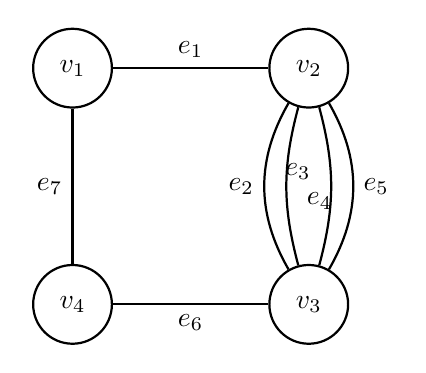
\begin{tikzpicture}[thick,
      main/.style = {draw, circle, minimum size=10mm},
      auto]
    % nodes
    \node[main] (1) at (0, 3) {$v_1$};
    \node[main] (2) at (3, 3) {$v_2$};
    \node[main] (3) at (3, 0) {$v_3$};
    \node[main] (4) at (0, 0) {$v_4$};

    % directed edges
    \draw (1) to node[above] {$e_1$} (2);
    \draw (2) to[bend right=30] node[left] {$e_2$} (3);
    \draw (2) to[bend right=15] node[right=-1.5mm, pos=.4] {$e_3$} (3);
    \draw (2) to[bend left=15] node[left=-1.5mm, pos=.6] {$e_4$} (3);
    \draw (2) to[bend left=30] node[right] {$e_5$} (3);
    \draw (3) to node[below] {$e_6$} (4);
    \draw (4) to node[left] {$e_7$} (1);
  \end{tikzpicture}
  \caption{A sample multigraph (opposite to a simple graph)}
  \label{fig:con-graph}
\end{figure}

\subsubsection{Seven Bridges of Königsberg}\label{subsubsec:con-seven-bridges}

Graph theory has been booming since 17th to 19th centuries.\footnote{In 1736, Leonhard Euler published a paper related to the Seven Bridges of Königsberg. This paper is regarded as the first paper in the history of graph theory, collected in \textit{Graph Theory, 1736--1936}, first published in 1976.} The initiation is the seven bridges problem in Prussia (now Russia).

In this problem, there are seven bridges among two mainlands and two islands on the Pregel river. The goal is to find a path to traverse all bridges exactly once and back to the starting point. See \cref{subsec:con-path} for more info about a path.

We have a graph as follows, shown in \cref{fig:con-seven-bridge}.
% ref: https://stackoverflow.com/a/33801400
\begin{equation*}
  G =
  \left(
  \begin{array}{l}
    \{ w,\, x,\, y,\, z \},                        \\
    \{ \foreach \i in {1,...,6} {e_\i,\, } e_7 \}, \\
    \{ wx,\, wx,\, wz,\, wz,\, wy,\, xy,\, yz \}
  \end{array}
  \right)
\end{equation*}

\begin{figure}[ht]
  \centering
  \begin{subfigure}{0.35\textwidth}
    \centering
    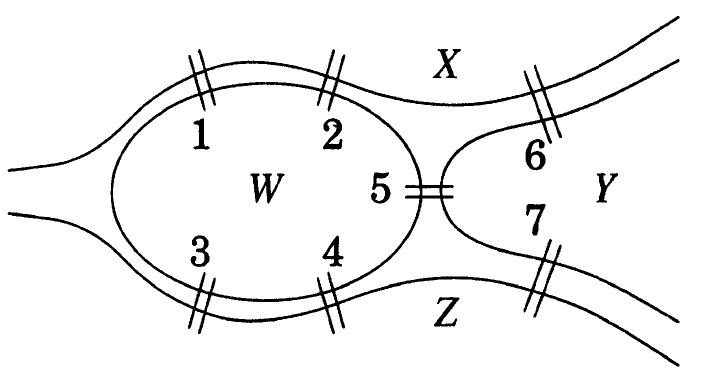
\includegraphics[width=\textwidth]{con-seven-bridge-original}
    \caption{Original version.}
    \label{fig:con-seven-bridge-original}
  \end{subfigure}
  \hspace{.1\textwidth}
  \begin{subfigure}{0.25\textwidth}
    \centering
    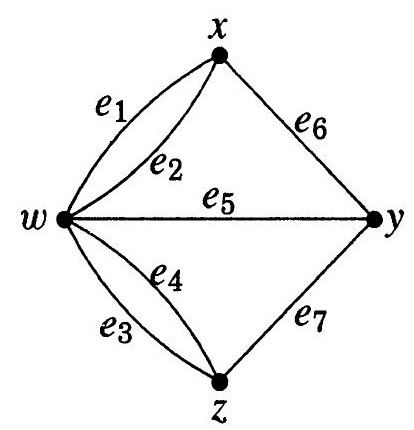
\includegraphics[width=\textwidth]{con-seven-bridge-graph}
    \caption{Graph version.}
    \label{fig:con-seven-bridge-graph}
  \end{subfigure}
  \caption{Seven-bridge problem.}
  \label{fig:con-seven-bridge}
\end{figure}

There are three principles related to the seven-bridge problem. You could try to list them on your own in advance:
\begin{enumerate*}
  \item If the degree (the number of connected edges) of each vertex is \textbf{even}, there must be a path to traverse all edges exactly once from and to the same vertex for an arbitrary vertex.
  \item If there are exactly \textbf{two} odd-degreed vertices, saying A and B, there must be a path to traverse all edges exactly once from A to B, or from B to A.
  \item If there are more than two odd-degreed vertices, three is no path to traverse all edges exactly once.
\end{enumerate*}

In the exams, you need to show why some graphs have no feasible solution with these three principles rather than showing all possible solutions.

We will cover the proofs of these principles in later sections. % TODO: link to their proofs

\subsubsection{Graph Terminologies}

\begin{definition}{}{con-loop}
  (1.1.4. Definition in text)
  A \textbf{loop} (so-called \textbf{self-loop}) is an edge whose endpoints are equal.

  \textbf{Multiple edges} are edges having the same pair of endpoints, like edges between $v_2$ and $v_3$ in a multigraph like \cref{fig:con-graph}.

  A \textbf{simple graph} is a graph having no loops or multiple edges.

  When $u$ and $v$ are the endpoints of an edge, they are \textbf{adjacent} and are \textbf{neighbors}, written $u \leftrightarrow v$.
\end{definition}

Continuing from \cref{def:con-loop}, if we have a node without a visible edge from an to it on graph, we wouldn't say that there is a self-loop.

\begin{definition}{}{con-finite-null-graph}
  (1.1.6.* Remark and the paragraph above it in text\footnote{The asterisk symbol (*) in the textbook \textit{Introduction to Graph Theory} means optional material that is not used later and can be skipped.})
  A \textbf{finite graph} has finite vertex set and edge set.

  A \textbf{null graph} (order-zero graph) has empty vertex set, and thus has empty edge set. Sometimes a null graph refers to an empty graph.

  An \textbf{empty graph} (edgeless graph) has finite vertex set and \textbf{empty} edge set.

  As for an \textbf{infinite graph}, it is usually used in Astronomy for infinite number of planets.
\end{definition}

Notice that in most cases, unless specified, we treat a graph as a simple and finite graph. In some cases, we consider null graphs and multigraphs.

\begin{definition}{}{con-complement}
  (1.1.8. Definition in text)
  The \textbf{complement} of a \textit{simple} graph $G$ is denoted by $\bar G$, which is the simple graph with vertex set $V(G)$ and edge set $E(\bar G)$ defined by $uv \in E(\bar G) \iff uv \notin E(G)$.

  A \textbf{clique} in a graph is a set of pairwise adjacent vertices. A single vertex is also a clique. However, it is controversial for a null graph to be a clique.

  An \textbf{independent set} (stable set) in a graph is a set of pairwise nonadjacent vertices. That is,
\end{definition}

\begin{figure}[ht]
  \centering
  \begin{subfigure}[t]{.3\textwidth}
    \centering
    % TODO: TikZ version
    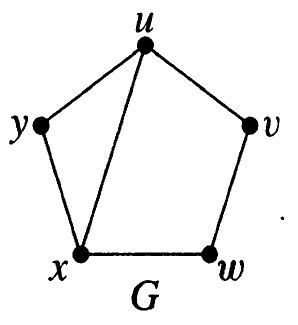
\includegraphics[width=\textwidth]{con-complement-before}
    \caption{The original graph $G$.}
    \label{fig:con-complement-before}
  \end{subfigure}
  \hspace{.1\textwidth}
  \begin{subfigure}[t]{.3\textwidth}
    \centering
    % TODO: TikZ version
    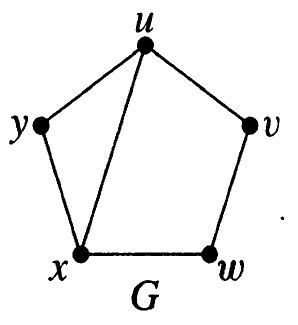
\includegraphics[width=\textwidth]{con-complement-before}
    \caption{The complement of graph $G$, denoted by $\bar G$.}
    \label{fig:con-complement-after}
  \end{subfigure}
  \caption{An example of complement of a graph. Also, vertices $u$, $x$ and $y$ in graph $G$ form a \textbf{maximal clique} of size 3 (three vertices); vertices $x$ and $w$ form a clique of size 2; vertex $u$ form a clique of size 1.}
  \label{fig:con-complement}
\end{figure}

For the complement in \cref{def:con-complement}, in brief, a complement of a graph $G$ consists of the same vertices of $G$ with all the edges \textit{not} in $G$ and without all the edges in $G$.

For the clique in \cref{def:con-complement}, note that a clique refers to a subset of vertices rather than edges or graphs.

When saying about a clique or an independent set, we usually need to find a maximal clique or a maximal independent set.

Finding a maximal clique and finding a maximal independent set are dual of each other. That is, finding a maximal clique in a graph $G$ (vertices $u,\, x,\, y$ in \cref{fig:con-complement-before}) is equal to finding an independent set in $\bar G$ (vertices $u,\, x,\, y$ in \cref{fig:con-complement-after}). \supp{If we find a maximal clique $C$ in $G$, since all vertices in $C$ are adjacent, they are all nonadjacent in $\bar G$, and it means a maximal independent set in $\bar G$.}

Finding a maximal clique, finding all cliques and finding a maximal independent set are all NP-complete problems.
And finding a maximal independent set is also a strongly NP-hard problem.

\begin{definition}{}{con-chromatic}
  (1.1.12. Definition in text)
  \textbf{Chromatic number} of a graph $G$, denoted by $\chi (G)$, is the \textit{minimum number of colors} needed to label the vertices so that adjacent vertices receive different colors.
\end{definition}

For \cref{def:con-chromatic}, that is, if two vertices has an edge between, these two vertices cannot have the same color. For a tree (because it's bipartite as shown in \cref{prop:con-bipartite-tree}), its chromatic number is 2. For a graph without edges, its chromatic number is 1.

For any finite graph (\cref{def:con-finite-null-graph}), we can find its chromatic number given that the colors can be hard for humans to distinguish (like \#FF1234 and \#FF1235 pixel values).

\supp{Chromatic numbers The complexity of finding a chromatic number is an open problem. It is likely NP-complete or NP-hard, but we couldn't find a way to reduce it to an NP-complete problem.}

\subsubsection{Bipartite Graphs}

\begin{definition}{}{con-bipartite}
  (1.1.10. Definition and 1.1.12. Definition in text)
  A graph $G$ is \textbf{bipartite} if $V(G)$ is the union of two disjoint (possibly empty) \textit{independent sets} called \textbf{bipartite sets} of $G$.

  For three disjoint independent sets, $G$ is \textbf{tripartite}.

  For $k$ disjoint independent sets, $G$ is $k$-partite (generally speaking, multipartite), where $k \in \set{ i : i \in \N \land i \geq 3}$.
\end{definition}

\begin{figure*}[ht]
  \centering
  \begin{subfigure}{.4\textwidth}
    \centering
    \bipartitegraphwithlabels
    \caption{A bipartite graph}
    \label{fig:con-bipartite}
  \end{subfigure}
  \hspace{.1\textwidth}
  \begin{subfigure}{.4\textwidth}
    \centering
    \tripartitegraph
    \caption{A tripartite graph.}
    \label{fig:con-tripartite}
  \end{subfigure}
  \caption{Bipartite and tripartite graphs.}
  \label{fig:con-bipartite-tripartite}
\end{figure*}

In \cref{fig:con-bipartite}, only people can get paid for jobs; people cannot get people (having no relation); jobs cannot get jobs. Thus, the following graph is a \textbf{bipartite graph}.

However, it is possible for all the people here to get no offers (jobs). This is a special case you need to consider in exams.

In a rooted tree like \cref{fig:con-rooted-tree}, you are able to see the children and parents of nodes, so you can find a root. In an unrooted tree like \cref{fig:con-unrooted-tree}, you couldn't. % TODO: link to tree

\begin{figure}[ht]
  \centering
  \begin{subfigure}[t]{.2\textwidth}
    \centering
    % TODO: TikZ version
    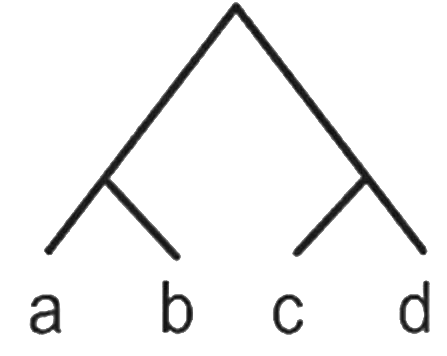
\includegraphics[width=\textwidth]{con-rooted-tree}
    \caption{A rooted tree}
    \label{fig:con-rooted-tree}
  \end{subfigure}
  \hspace{.1\textwidth}
  \begin{subfigure}[t]{.2\textwidth}
    \centering
    % TODO: TikZ version
    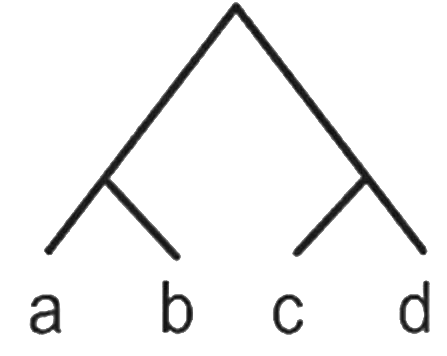
\includegraphics[width=.8\textwidth]{con-unrooted-tree}
    \caption{An unrooted tree}
    \label{fig:con-unrooted-tree}
  \end{subfigure}
  \hspace{.1\textwidth}
  \begin{subfigure}[t]{.3\textwidth}
    \centering
    % TODO: TikZ version
    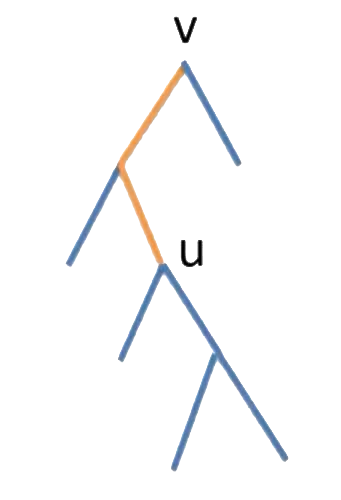
\includegraphics[width=.5\textwidth]{con-bipartite-tree}
    \caption{An illustration to prove that a rooted tree is a bipartite graph}
    \label{fig:con-bipartite-tree}
  \end{subfigure}
  \caption{Examples of rooted trees and unrooted trees}
  \label{fig:con-rooted-unrooted-trees}
\end{figure}

In programming, you could use linked lists to store a tree, but in graph theory, rooted and unrooted trees have different meaning.

\begin{proposition}{}{con-bipartite-tree}
  A tree (either rooted or unrooted one) is bipartite.
\end{proposition}

\textbf{Proof} of \cref{prop:con-bipartite-tree}:
Our goal is to find a partition of two disjoint independent sets.
Let $v$ be the root of a tree (we could pick any node, but this node is fixed in the following proof), and let $u$ be an arbitrary node in the tree.
We can find the distance between $v$ and $u$, and such a distance is a non-negative integer ($\N \cap \{ 0 \}$).
We partition all nodes in the tree into two sets: a set $S_e$ for all nodes with even distances to $v$, including $v$ itself; a set $S_o$ for all nodes with odd distances to $v$.
There is no exception for non-even and non-odd distances.
Since $S_e$ and $S_o$ are disjoint independent sets, the tree is a bipartite graph.
This applies to all trees including rooted and unrooted trees.

So, for a coloring problem on a tree, we could apply the same technique above to find two independent sets to solve the problem. We could also prove \cref{prop:con-bipartite-tree} with a coloring problem. % TODO: link to coloring problem

Note that some proofs are pretty simple, but it doesn't mean that they wouldn't be in exams.

Some comments for bipartite graphs:
\begin{enumerate}
  \item \label{enum:con-bipartite-odd} A bipartite graph is a graph with no odd length cycle. That is, there doesn't exist a path to traverse some vertices along edges and back to the starting point with odd number of edges. For a graph with no possible cycles or with only even length cycles, such a graph is also bipartite. \supp{A bonus problem is as follows. Proove that a graph is not bipartite if it has one or more \textit{arbitrary} (3, 5, 7, etc.) odd length cycles. However, in 2024 spring, announced in 2024-03-08, the bonus problem changed to a program homework with different topics.}

  \item Another ways to define an $n$-vertex tree $G$, where $n \geq 1$:
        \begin{enumerate}
          \item $G$ satisfies any two of the following three rules:
                \begin{enumerate}
                  \item $G$ is connected. (See \cref{fig:con-connected-graph-interlude} for the illustration of connected and unconnected graphs. And see \cref{def:con-connected} for the definition.)
                  \item $G$ has "$n - 1$" edges.
                  \item $G$ has no cycles. Note that a self-loop is a cycle.
                \end{enumerate}
          \item $G$ has no loops, and for each $u,\, v \in V(G)$, there exists exactly one $u,\, v$-path. (This rule is sufficient to show that $G$ is a tree, for the later part shows the three rules above.) % TODO: link to their proofs
        \end{enumerate}
\end{enumerate}

Note that a graph $G$ with "$n - 1$" edges doesn't mean $G$ is connected. For example, a graph with two components: one is a triangle with three vertices and three edges, and the other one is an isolated graph with a vertex. Such a graph is 4 vertices with 3 edges, but is disconnected.

\supp{In the above-mentioned definition of a tree, we could pick two rules in three because in their proofs, they show that any two satisfied rules imply the other rule in a circular way.}

\begin{figure}[ht]
  \centering
  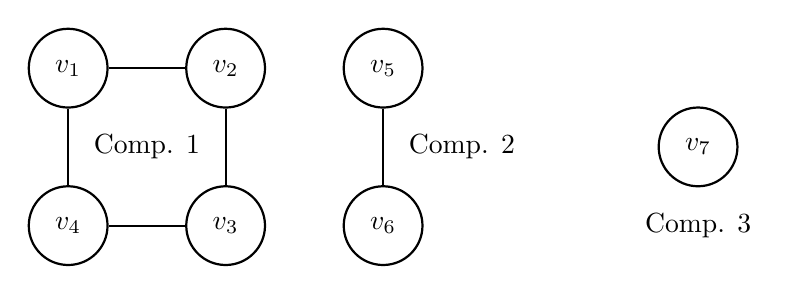
\begin{tikzpicture}[thick,
      main/.style = {draw, circle, minimum size=10mm},
      auto]
    % nodes
    \node[main] (1) at (0, 2) {$v_1$};
    \node[main] (2) at (2, 2) {$v_2$};
    \node[main] (3) at (2, 0) {$v_3$};
    \node[main] (4) at (0, 0) {$v_4$};
    \node at (1, 1) {Comp. 1};

    \node[main] (5) at (4, 2) {$v_5$};
    \node[main] (6) at (4, 0) {$v_6$};
    \node at (5, 1) {Comp. 2};

    \node[main] (7) at (8, 1) {$v_7$};
    \node at (8, 0) {Comp. 3};

    % undirected edges
    \draw (1) -- (2) -- (3) -- (4) -- (1);
    \draw (5) -- (6);

  \end{tikzpicture}
  \caption{An unconnected graph with three sub-components (connected subgraph). If we removes vertices $v_5$, $v_6$ and $v_7$, we would have a connected graph with exactly one component. In brief, in a connected graph, each two nodes $u,\, v$ has at least one path. See \cref{def:con-connected} for the definition of connected and unconnected graphs.}
  \label{fig:con-connected-graph-interlude}
\end{figure}

\subsection{Paths, Cycles and Trails}\label{subsec:con-path}

\begin{definition}{}{con-path-cycle}
  (1.1.15. Definition in text)
  A \textbf{path} is a (ordered) \textbf{sequence} of \textit{distinct} vertices such that any two consecutive vertices are adjacent. We call $v_0$ and $v_k$ the endpoints of the path $\anglebrackets{v_0,\, v_1,\, \ldots,\, v_k}$.

  A \textbf{cycle} is a sequence of vertices, where all vertices except the last vertex are distinct, and the two endpoints are equal, such that any two consecutive vertices are adjacent. For example, $\anglebrackets{v_0,\, v_1,\, \ldots,\, v_k,\, v_0}$.
\end{definition}

In \cref{def:con-path-cycle}, note that a path or a cycle refers to a set of vertices instead of edges, although any two consecutive vertices being adjacent implies edges.

There are examples for \cref{def:con-path-cycle} in \cref{fig:con-path-cycle}. Note that in \cref{fig:con-cycle}, the intersection point of edges $xb$ and $yz$ is not a vertex.

In \cref{fig:con-path}, reversing the order of vertices in the given path gives another path by definition. The vertex sequence matters. Same for \cref{fig:con-cycle}; starting from $a$ back to $a$ and starting from $b$ back to $b$ yield two different cycles, and if you go in the other direction, you have another two different cycles in definition.

\begin{figure}[ht]
  \def \nodelist {
    \node[main] (x) at (0, 1.5) {$x$}
    node[main] (y) at (0, 0) {$y$}
    node[main] (z) at (1.5, 1.5) {$z$}
    node[main] (b) at (1.5, 0) {$b$}
    node[main] (a) at (3, 0.75) {$a$};}

  \centering
  \begin{subfigure}{.3\textwidth}
    \centering
    \begin{tikzpicture}[
        main/.style = {draw, circle}
      ]
      \nodelist
      \draw (x) -- (b) -- (a) -- (z) -- (y);
    \end{tikzpicture}
    \caption{$\anglebrackets{x,\, b,\, a,\, z,\, y}$ is a path.}
    \label{fig:con-path}
  \end{subfigure}
  \begin{subfigure}{.3\textwidth}
    \centering
    \begin{tikzpicture}[
        main/.style = {draw, circle}
      ]
      \nodelist
      \draw (x) -- (b) -- (a) -- (z) -- (y) -- (x);
    \end{tikzpicture}
    \caption{$\anglebrackets{a,\, b,\, x,\, y,\, z,\, a}$ is a cycle.}
    \label{fig:con-cycle}
  \end{subfigure}

  \caption{Examples for a path and a cycle for \cref{def:con-path-cycle}.}
  \label{fig:con-path-cycle}
\end{figure}

\begin{definition}{}{con-subgraph}
  (1.1.16. Definition in text)
  A \textbf{subgraph} of $G$ is a graph $S$ such that $\ldots$
  \begin{enumerate*}
    \item $V(S) \subseteq V(G)$ and
    \item $E(S) \subseteq E(G)$ and
    \item the assignment of endpoints to edges in $S$ is the same in $G$.
  \end{enumerate*}

  The third requirement means that for vertices $u$ and $v$ in $S$, there won't be an edge $uv$ if there is no such an edge in $G$.

  We denote $S \subseteq G$ for a subgraph of a graph $G$.
\end{definition}

For \cref{def:con-subgraph}, in other words, if $S \subseteq G$, all vertices and edges in $S$ are in $G$ without introducing new vertices or edges. Later, we will cover induced subgraphs, which pose a constraint on edges. % TODO: link to induced subgraphs

\begin{definition}{Connected graphs}{con-connected}
  (1.1.16. Definition in text)
  A graph $G$ is \textbf{connected} if each pair of vertices in $G$ belongs to a path. Otherwise, $G$ is \textbf{disconnected}.
\end{definition}

For \cref{def:con-connected}, in other words, if a graph $G$ is connected, you can find a path from any one vertex to each other vertices. % TODO: link to its definition with components

See \cref{fig:con-connected-unconnected} for the examples of \cref{def:con-connected}.

\begin{figure}[ht]
  % ref using inner sep to set maximum size: https://tex.stackexchange.com/a/228365
  % ref for every node: https://tex.stackexchange.com/a/78718
  \centering
  \begin{subfigure}[t]{.4\textwidth}
    \centering
    \tripartitegraph
    \caption{A connected graph.}
    \label{fig:con-connected}
  \end{subfigure}
  \begin{subfigure}[t]{.4\textwidth}
    \centering
    \bipartitegraph
    \caption{An unconnected graph (with two connected subgraphs) even though it is bipartite (\cref{def:con-bipartite}).}
    \label{fig:con-unconnected}
  \end{subfigure}
  \caption{Examples for a connected graph and an unconnected graph.}
  \label{fig:con-connected-unconnected}
\end{figure}

\subsection{Graph Isomorphism}\label{subsec:con-graph-isomorphism}

\begin{definition}{}{con-adj}
  (1.1.17. Definition in text)
  Let $G$ be a loopless graph with vertex set $V(G) = \set{ v_1,\, v_2,\, \ldots,\, v_n}$ and edge set $E(G) = \set{ e_1,\, e_2,\, \ldots,\, e_m}$:

  \begin{enumerate}
    \item The \textbf{adjacency matrix} of $G$, written $A(G)$, is an $n$-by-$n$ matrix where entry $a_{i,j}$ is the number of edges in $G$ with endpoints $\set{v_i,\, v_j}$.
    \item The \textbf{incidence matrix} of $G$, written $M(G)$, is an $n$-by-$m$ matrix where entry $m_{i,j}$ is 1 if $v_i$ is an endpoint of edge $e_j$. Otherwise, $m_{i,j}$ is 0.
  \end{enumerate}

  A vertex $v$ is \textbf{incident} with an edge $e$ if $v$ is an endpoint of $e$. (cf. \textit{adjacent} in \cref{def:con-loop}: $u$ and $v$ are adjacent/neighbors if $u$ and $v$ are the endpoints of an edge $e$.)

  The \textbf{degree} of a vertex $v$ in a loopless undirected graph is the number of incident (ingoing) edges of $v$. In an undirected graph, an edge is both ingoing and outgoing to both its endpoints.

  In a directed graph, the \textbf{indegree} of a vertex $v$ is the number of ingoing edges (arrows); the \textbf{outdegree} of a vertex $v$ is the number of outgoing edges (tails).
\end{definition}

In \cref{def:con-adj}, in brief, the adjacency matrix records the number of edges between each two vertices; the incidence matrix records the endpoints of each edge. See \cref{fig:con-adj} for some examples.

(1.1.18 Remark) The adjacency matrix of a simple graph consists of 0 and/or 1. In a simple undirected graph, the adjacency matrix is always \textbf{symmetric} ($A(G) = A(G)^\trans$) with all zeros on the diagonal.

In a finite graph, the incidence matrix consists of 0 and/or 1, and each vertex has a degree (at least 0).

\begin{figure}[ht]
  \centering
  % TODO: TikZ and blkarray versions
  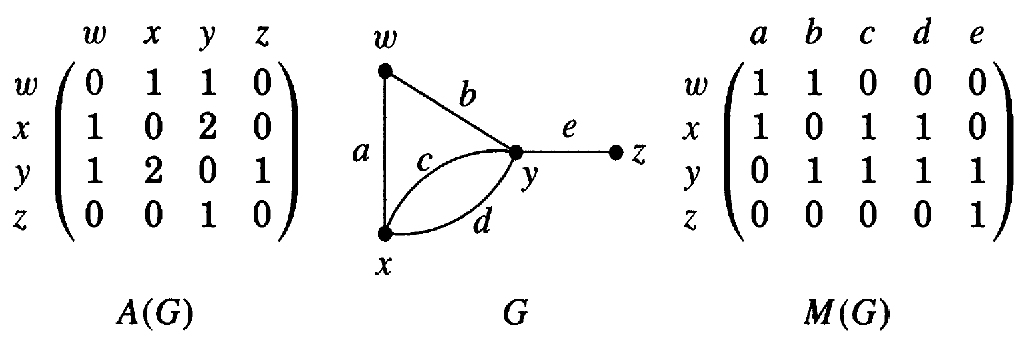
\includegraphics[width=.8\textwidth]{con-adj}
  \caption{A graph $G$ with its adjacency matrix $A(G)$ and incidence matrix $M(G)$. $a_{i,j}$ in $A(G)$ is $\set{v_i,\, v_j}$ in $G$.}
  \label{fig:con-adj}
\end{figure}

\begin{definition}{}{con-isomorphism}
  (1.1.20. Definition in text)
  An \textbf{isomorphism} from a \textbf{simple graph} $G$ to a \textbf{simple graph} $H$ is a \textbf{bijection function} (equivalent relation; \cref{def:intro-equiv-relation}) $\func{f}{V(G)}{V(H)}$ such that $uv \in E(G) \iff f(u)f(v) \in E(H)$. See \cref{def:con-loop} for the definition of simple graphs.

  We say "$G$ is \textbf{isomorphic to} $H$", written $G \isomorphicto H$, if there is an isomorphism from $G$ to $H$.
\end{definition}

You could recall three special function, including a bijective function as shown in \cref{fig:intro-special-functions}.
\reusefigure[ht]{fig:intro-special-functions}

For \cref{def:con-isomorphism}, in other words, a graph $G$ is isomorphic to a graph $H$ if and only if there exists a bijection function $\func{f}{V(G)}{V(H)}$, where $V(G)$ and $V(H)$ are vertices sets of $G$ and $H$ respectively, such that for every edge $uv$ in $G$, there is a corresponding edge $f(u)f(v)$ in $H$, and vice versa, without introducing additional vertices or edges.

For two isomorphic graphs $G$ and $H$, they may look different by human eyes. And note that a prerequisite for isomorphism is the same number of vertices and the same number of degrees. With different numbers of vertices or a degree that is absent one graph, the two graphs cannot be isomorphic. But with the same number of vertices and the same number of degrees, we still need a bijection function to prove the isomorphism from one graph to the other one.

See \cref{fig:con-isomorphism} for an example. In this example, we could see that vertices $w,\, z$ may correspond to $c,\, a$; and $x,\, y$ to $b,\, d$.

\begin{figure}[ht]
  \centering
  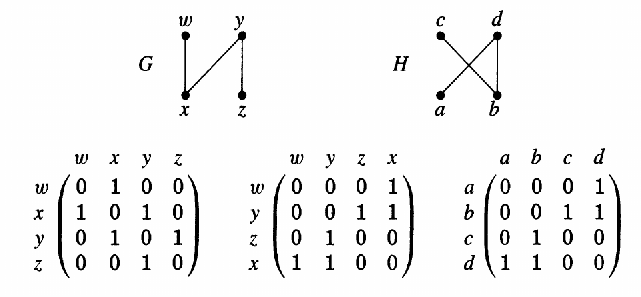
\includegraphics[width=.7\textwidth]{con-isomorphism}
  \caption{An example that $G$ is isomorphic to $H$. The following three matrices are adjacency matrices.}
  \label{fig:con-isomorphism}
\end{figure}

\supp{
  In programming, to determine whether graphs $G$ and $H$ are isomorphic to each other, we could build adjacency matrices for these two graphs (matrices 1 and 3 in \cref{fig:con-isomorphism}) respectively after fixing the order of vertices in $H$ to $a,\, b,\, c,\, d$ and choosing an order of vertices in $G$. Later, if the two adjacency matrices are different, change the order of vertices in $G$ to the other untested order, saying $w,\, y,\, z,\, x$, and then build the adjacency matrix of $G$ according to the new order. Note that for a new order of vertices, you cannot simply swap columns in the matrix because the row order changes as well. Once the adjacency matrices of $G$ and $H$ are identical like the matrices 2 and 2 in \cref{fig:con-isomorphism}, we could find the bijection function for vertex sets of $G$ and $H$. In \cref{fig:con-isomorphism}, vertices $w,\, y,\, z,\, x$ in $G$ correspond to vertices $a,\, b,\, c,\, d$ in $H$ respectively.

  The complexity of graph isomorphism is an open problem. It is highly possible not a $P$ problem. By the say, the subgraph problem (determining whether a smaller graph is isomorphic to some subgraph(s) in a larger graph) is NP-complete.

  A bonus problem (not in 2024 spring) is as follows. How do you define two multigraphs (including the cases of multiple edges and loops; see \cref{def:con-loop} for definition) are isomorphism? We need definition rather than proofs. Isomorphism in multigraphs is possible in real world. There is no commonly approved definition, but many different definitions you can reference. Note that graph (multigraph) isomorphism always follows the principle of bijection (one-to-one correspondence). Your answer has to be handwritten in Chinese clearly, possibly using the same ideas from references.
}

Recall \cref{def:intro-equiv-relation} as follows.
\recall[\sectionprefix]{intro-equiv-relation}

\supp{Friendship relation is not always an equivalence relation. Relation in law is an equivalence relation. An equivalence relation in graph theory is commonly used to collect all sets with the same relation.}

\begin{proposition}{}{con-iso-equiv}
  (1.1.24. Proposition in text)
  The isomorphism relation is an equivalence relation on the set of \textbf{simple} graphs.
\end{proposition}

\textbf{Proof} of \cref{prop:con-iso-equiv}:

\begin{enumerate}
  \item Reflexive: $G \isomorphicto G$. (A graph and itself have isomorphism relation.)
  \item Symmetric: $uv \in E(G) \iff f(u)f(v) \in E(H)$ yields $xy \in E(H) \iff f^{-1}(x)f^{-1}(y) \in E(G)$. So, $G \isomorphicto H \iff H \isomorphicto G$. Consider $f$ and its inverse ($f^{-1}$) to be bijection functions.
  \item Transitive:
        \begin{enumerate}
          \item See \cref{fig:con-iso-equiv} for the illustration.
          \item Let $\func{f}{V(F)}{V(G)}$ and $\func{g}{V(G)}{V(H)}$ be two isomorphism relation functions.
          \item Given $uv \in E(F) \iff f(u)f(v) \in E(G)$ and $xy \in E(G) \iff g(x)g(y) \in E(H)$ by definition, since $f$ is an isomorphism, for every $xy \in E(G)$ we can find $uv \in E(G)$ such that $f(u) = x$ and $f(v) = y$.
          \item The last statement yields $uv \in E(F) \iff g(f(u))g(f(v)) \in E(H)$, where $f(u) = x$ and $f(v) = y$.
          \item Thus, the composition $g \composition f$ is an isomorphism from $F$ to $H$.
          \item We have proved that $F \isomorphicto G$ and $G \isomorphicto H$ together imply $F \isomorphicto H$.
        \end{enumerate}
\end{enumerate}

\begin{figure}[htbp]
  \def\hoffset{3cm}%
  \def\voffset{1.2cm}%
  \def\domain#1#2{\draw[fill=#2] (\hoffset * #1, 0) ellipse (1cm and 2cm)}%
  \def\elements#1#2#3#4{
    \node[main] (#3) at (\hoffset * #1, \voffset) {$#3$}
    node[main] (#4) at (\hoffset * #1, 0) {$#4$}
    node at (\hoffset * #1, -\voffset) {$#2$};
    \draw[edge] (#3) -- (#4)
  }
  \centering
  \begin{tikzpicture}[
      main/.style = {draw, circle, fill=white, minimum size=.8cm},
      edge/.style = {thick},
      trans/.style = {dashed, -Latex}
    ]
    \foreach \d/\c in {1/yellow, 2/green, 3/cyan}
    \domain{\d}{\c};

    \foreach \i/\d/\a/\b in {1/F/u/v, 2/G/x/y, 3/H/a/b}
    \elements{\i}{\d}{\a}{\b};

    \foreach \a/\f/\x in {u/f/x, v/f/y, x/g/a, y/g/b}
    \draw[trans] (\a) to node[midway, above] {$\f$} (\x);
  \end{tikzpicture}
  \caption{An illustration for the transitive property of isomorphism in \cref{prop:con-iso-equiv}. Given $F \isomorphicto G$ by a function $f$ and $G \isomorphicto H$ by a function $g$, $f \composition g$ is also a bijection function and an isomorphism.}
  \label{fig:con-iso-equiv}
\end{figure}

If we have some graphs isomorphic to one another; that is, satisfying the proofs of \cref{prop:con-iso-equiv} for each one, each two, each three of graphs, we could use a set to collect all of such graphs. Such a set is an \textbf{equivalence class} (\textbf{equivalence set}). \supp{A star and a pentagon are in the same equivalence class.}

\begin{definition}{}{con-complete}
  (1.1.27. Definition in text)
  A \textbf{complete graph} $K_n$ is a simple graph whose vertices are \textbf{pairwise} adjacent; $K_n$ denotes the \textbf{unlabeled} complete graph with $n$ vertices.

  A \textbf{complete bipartite graph} $K_{r,s}$ or \textbf{biclique} is a simple bipartite graph such that two vertices are adjacent iff. they are in different partite sets.
\end{definition}

For \cref{def:con-complete}, a complete graph with $n$ vertices is $K_n$ rather than $C_n$, which refers to a cycle. $P_n$ is a path. You couldn't rename them, for they are well-known in graph theory.

A complete bipartite graph is not a complete graph. Nonetheless, $K_{r,s}$ is a subgraph of $K_n$, given $r \leq n$ and $s \leq n$.

$C_3$ is a subgraph of $K_5$. In a $K_5$, there are $C_5^3 = 10$ (combination) distinct $C_3$. However, in $K_{2,3}$, there is no $C_3$, which is an odd-length cycle. See Theorem 1.2.18, comment \ref{enum:con-bipartite-odd} in \cpageref{enum:con-bipartite-odd} and \cref{rem:intro-equal-sets} in \cpageref{rem:intro-equal-sets} for the definition of bipartite graphs. % TODO: link to Theorem 1.2.18

\begin{figure}[htbp]
  \centering
  \begin{subfigure}[t]{.4\textwidth}
    \centering
    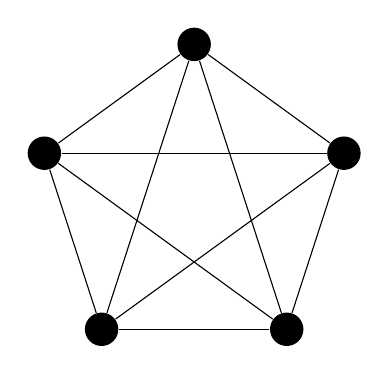
\begin{tikzpicture}[every node/.style = {circle, fill=black, inner sep=1.5mm}]
      \def\num{5}%
      \def\degoffset{360 / \num}%
      \foreach \i in {1,...,\num}{
          \node (\i) at (\degoffset * \i + 90 : 2) {};
          \foreach \j in {1,...,\i}{
              \ifthenelse{\i = \j}{}{
                \draw (\i) -- (\j);
              }
            }
        }
    \end{tikzpicture}
    \caption{$K_5$: A complete graph with 5 vertices.}
    \label{fig:con-complete}
  \end{subfigure}
  \hspace{2cm}
  \begin{subfigure}[t]{.4\textwidth}
    \centering
    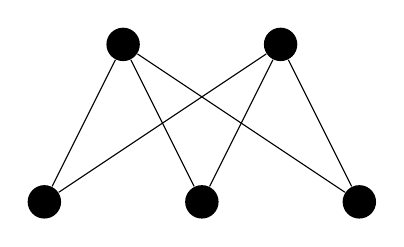
\begin{tikzpicture}[every node/.style = {circle, fill=black, inner sep=1.5mm}]
      \def\numi{2}%
      \def\numj{3}%
      \node foreach \i in {1,...,\numi} (a\i) at (2 * \i - 2, +1) {};
      \node foreach \j in {1,...,\numj} (b\j) at (2 * \j - 3, -1) {};

      \foreach \i in {1,...,\numi}
      \foreach \j in {1,...,\numj}
      \draw (a\i) -- (b\j);
    \end{tikzpicture}
    \caption{$K_{2,3}$: A complete bipartite graph with 2 and 3 vertices in partite sets respectively.}
    \label{fig:con-complete-bipartite}
  \end{subfigure}
  \caption{Examples for complete graphs and bipartite complete graphs.}
  \label{fig:con-complete-bipartite-full}
\end{figure}

\begin{example}{}{con-relation}
  (1.1.30. Example in text)
  Given the four figures as shown in \cref{fig:con-relation}, please answer the following questions.
  \begin{enumerate}
    \item \textbf{Question}: Which graphs are isomorphic to each other or one another?\\\textbf{Answer}: $G_1,\, G_2,\, G_4$ form an equivalence class. $G_3$ forms the other equivalence set.

    \item \textbf{Question}: Are the complement graphs of two isomorphic (simple) graphs also isomorphic?\\\textbf{Answer}: Yes.
  \end{enumerate}
\end{example}

\begin{figure}[htbp]
  \newcommand\quartersubfigure[4][width=.8\textwidth]{%
    \begin{subfigure}[t]{.2\textwidth}%
      \centering%
      \includegraphics[#1]{#2}%
      \caption{#3}%
      \label{#4}%
    \end{subfigure}%
  }%
  \centering
  \quartersubfigure[width=.6\textwidth]{con-relation-g1}{$G_1$ ($K_{3,3}$)}{fig:con-relation-g1}
  \quartersubfigure{con-relation-g2}{$G_2$ (hexagon)}{fig:con-relation-g2}
  \quartersubfigure{con-relation-g3}{$G_3$}{fig:con-relation-g3}
  \quartersubfigure{con-relation-g4}{$G_4$}{fig:con-relation-g4}
  \caption{Four figures for the relation examples.}
  \label{fig:con-relation}
\end{figure}

Detailed answer to question 1 in \cref{ex:con-relation}:
\begin{enumerate*}
  \item Suppose that $G_1$ and $G_2$ are an isomorphism.
  \item Select a fixed vertex mapping from $G_1$ to $G_2$, saying $u$ to 1.
  \item Since $u$ has three edges to vertices $x$, $y$, and $z$ respectively, in $G_2$, they such three vertices are mapped to 2, 4 and 6.
  \item After finding all one-to-one correspondences, you can show that $G_1$ is isomorphic to $G_2$.
  \item In the other way, since $G_1$ is $K_{3,3}$, if we find a way to convert $G_2$ to $K_{3,3}$, we can also show the isomorphism. For example, two disjoint and independent sets $\{ 1,\, 3,\, 5 \}$ and $\{ 2,\, 4,\, 6 \}$.
  \item In $G_3$, we can easily find two $C_3$ (as odd-length cycles), so $G_3$ is not bipartite; thus, cannot be isomorphic to $G_1$ or $G_2$. $C_3$ is isomorphic to $K_3$; $K_3$ is not a subgraph of $K_{3,3}$.
\end{enumerate*}

Detailed answer to question 2 in \cref{ex:con-relation}:
\begin{enumerate*}
  \item For vertices in a complement graph, they are identical to the original graph.
  \item By definition of a complement graph in \cref{def:con-complement}, the two complement graphs have the same relation. This required a proof, though.
  \item For example, the complement of $G_1$, $G_2$ or $G_4$ is a disconnected graph with two $C_3$ (triangle). The complement of $G_3$ is a $C_6$.
  \item In conclusion, you cannot know whether a complement graph is disconnected or connected given the original graph connected or disconnected.
  \item The complement of a \textbf{complete} bipartite graph with at least two vertices always has two components. Generally, the complement of a bipartite graph doesn't always a disconnected graph.
  \item You need to understand the logics thoroughly to pass exams.
\end{enumerate*}

\begin{definition}{}{con-self-comp}
  A graph is \textbf{self-complementary} if it is isomorphic to its complement.

  A \textbf{decomposition} of a graph is a list of subgraphs such that each edge appears in exactly one subgraph in ths list.

  An $n$-vertex graph $H$ is self-complementary \textbf{iff.} $K_n$ has a decomposition consisting of two copies of $H$. (Not proved in text)
\end{definition}

Consider only the thick edges in \cref{fig:con-self-comp-pentagon} as a graph; such a graph is self-complementary. However, $K_5$ is not self-complementary, for the complement of $G_5$ has no edges.

In exams, you may be asked whether $K_4$ can be decomposed by some copies of $P_3$ like \cref{fig:con-self-comp-rectangle}, where the numbers 4 and 3 may change. Note that each edge in the decomposition must appear exactly once. As shown in \cref{fig:con-self-comp-heptagon}, you could decompose $K_7$ with 7 copies of $C_3$. As shown in \cref{fig:con-self-comp-pentagon-cdot}, you could decompose $K_6$ with 6 copies of $P_4$.

You might have noticed that to decompose a graph $G$ by some copies of $H$, the number of edges in $G$ must be multiples of those in $H$. However, this is not sufficient to decompose $G$ in that way. For example, you couldn't decompose $K_5$ in \cref{fig:con-self-comp-pentagon} with two kites in \cref{fig:con-graph-menageries}.

\begin{figure}[htbp]
  \def \nodesize {.8mm}%
  \def \shapesize {1.5cm}%
  \def \subfiguresize {.4\textwidth}%
  \def \hseparation {.1\textwidth}%
  \centering
  \begin{subfigure}[t]{\subfiguresize}
    \centering
    \begin{tikzpicture}[every node/.style = {circle, fill=black, inner sep=\nodesize}]
      \def\num{5}%
      \def\degoffset{360 / \num}%
      % node 1 at topmost corner; count nodes clockwise
      % \degoffset * -(\i - 1) means clockwise offset degrees from node 1
      % + 90 to rotate left 90 degrees to make node 1 at top
      \node foreach \i in {1,...,\num} (\i) at (-\degoffset * \i + \degoffset + 90 : \shapesize) {};
      \foreach \i in {1,...,\num} {
          \draw[evaluate={\j=int(1+mod(\i, \num));}, ultra thick] (\i) -- (\j);
          \draw[evaluate={\j=int(1+mod(\i+1, \num));}] (\i) -- (\j);
        }
    \end{tikzpicture}
    \caption{A decomposition of $K_5$ could be two 5-cycles $C_5$, including the thick one and inner star. (1.1.33. Example in text)}
    \label{fig:con-self-comp-pentagon}
  \end{subfigure}
  \hspace{\hseparation}
  \begin{subfigure}[t]{\subfiguresize}
    \centering
    \begin{tikzpicture}[every node/.style = {circle, fill=black, inner sep=\nodesize}]
      \def\num{4}%
      \def\degoffset{360 / \num}%
      % node 1 at top-left corner; count nodes clockwise
      % \degoffset * -(\i - 1) means clockwise offset degrees from node 1
      % + 135 to rotate left 135 degrees to make node 1 at top-left corner
      \node foreach \i in {1,...,\num} (\i) at (-\degoffset * \i + \degoffset + 135 : \shapesize) {};
      \draw[ultra thick] (4) -- (1) -- (2);
      \draw (1) -- (3) -- (4);
      \draw[dashed] (3) -- (2) -- (4);
    \end{tikzpicture}
    \caption{A decompose of $K_4$ could be three $P_3$, including the thick, normal and dashed ones. (1.1.33. Example in text)}
    \label{fig:con-self-comp-rectangle}
  \end{subfigure}

  \vspace{1em}

  \begin{subfigure}[t]{\subfiguresize}
    \centering
    \begin{tikzpicture}[every node/.style = {circle, fill=black, inner sep=\nodesize}]
      \def\num{7}%
      \def\degoffset{360 / \num}%
      % node 1 at topmost corner; count nodes clockwise
      % \degoffset * -(\i - 1) means clockwise offset degrees from node 1
      % + 90 to rotate left 90 degrees to make node 1 at top
      \node foreach \i in {1,...,\num} (\i) at (-\degoffset * \i + \degoffset + 90 : \shapesize) {};
      \draw[ultra thick] (1) -- (2) -- (4) -- (1);
      \draw (2) -- (3) -- (5) -- (2);
      \draw[dashed] (3) -- (4) -- (6) -- (3);
    \end{tikzpicture}
    \caption{A decomposition of $K_7$ could be 7 triangles $C_3$ by rotating the thick one through seven possible positions like the normal and dashed ones. (1.1.34.* Example in text)}
    \label{fig:con-self-comp-heptagon}
  \end{subfigure}
  \hspace{\hseparation}
  \begin{subfigure}[t]{\subfiguresize}
    \centering
    \begin{tikzpicture}[every node/.style = {circle, fill=black, inner sep=\nodesize}]
      \def\num{5}%
      \def\degoffset{360 / \num}%
      % node 1 at top-left corner; count nodes clockwise
      % \degoffset * -(\i - 1) means clockwise offset degrees from node 1
      % + 90 to rotate left 90 degrees to make node 1 at top
      \node foreach \i in {1,...,\num} (\i) at (-\degoffset * \i + \degoffset + 90 : \shapesize) {};
      \node (6) {};
      \draw[ultra thick] (6) -- (1) -- (3) -- (2);
      \draw (6) -- (2) -- (4) -- (3);
    \end{tikzpicture}
    \caption{To decompose $K_6$, you could place a vertex at the center of a pentagon, and constructing a $P_4$ with edges from each of (1) the outer $C_5$, (2) the inner star $C_5$ and (3) the edges involving the center vertex. By rotating the thick $P_4$ through 5 positions like the normal one, we get a decomposition of $K_6$ using 5 $P_4$. (1.1.34.* Example in text)}
    \label{fig:con-self-comp-pentagon-cdot}
  \end{subfigure}
  \caption{Examples of self-complementary graphs and decompositions of graphs.}
  \label{fig:con-self-comp}
\end{figure}

In \cref{fig:con-graph-menageries}, a claw is a biclique $K_{1,3}$, if we group the center vertex, and group the other vertices. A paw is a claw with an additional edge. A kite is $K_4$ without an edge. Exercises 1.1.6--8, 32, 34--37 in text discuss the characteristics of the four graphs on the top of \cref{fig:con-graph-menageries}. For example, the complements of these four graphs (triangle, claw, paw, kite) are disconnected.

\begin{figure}[htbp]
  \centering
  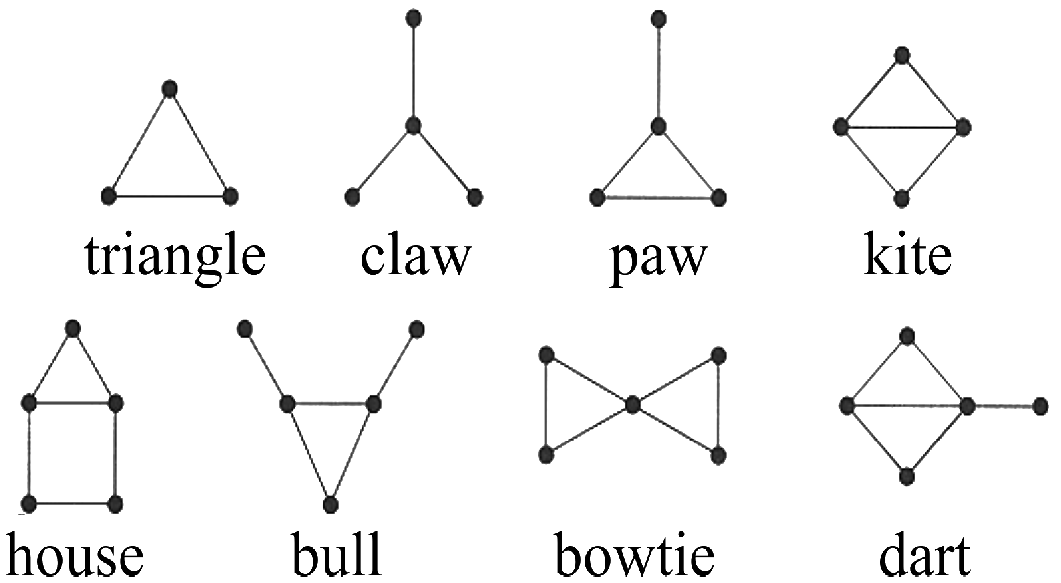
\includegraphics[width=.5\textwidth]{con-graph-menageries}
  \caption{Graph menageries}
  \label{fig:con-graph-menageries}
\end{figure}

\begin{definition}{}{con-petersen}
  (1.1.36. Definition in text)
  A \textbf{Petersen graph} (PG) is the \textbf{simple graph} whose vertices are the 2-element subsets of a 5-element set and whose edges are the pairs of \textbf{disjoint} 2-element subsets.

  The \textbf{girth} of a graph with a cycle is the length of its shortest cycle. A graph with no cycle has infinite girth.
\end{definition}

For a Petersen graph in \cref{def:con-petersen}, in other words, given a simple graph and any 5 elements (like 1--5 or a--e), if there are exactly two different elements (as an unordered set) chosen from the 5 elements on each vertex, and if the endpoints of each edge have distinct numbers, such a graph is a Petersen graph. For example, the leftmost graph in \cref{fig:con-petersen-examples}.

As you can see in the leftmost graph in \cref{fig:con-petersen-examples}, the topmost vertex has elements $\{ 1,\, 2, \}$; its neighbors has $\{ 4,\, 5 \}$, $\{ 3,\, 5 \}$, $\{ 3,\, 4 \}$ respectively. If any two neighbors of the topmost vertex are neighbors (there is a triangle in the graph), you couldn't choose 6 distinct elements out of 5 distinct elements.

For a graph with two cycles: a triangle $C_3$ and a rectangle $C_4$, the girth of that graph is 3, which is the length $C_3$. The minimal possible value of the girth of a graph is 1 in graphs with self-loops. Without a cycle in a graph, the length for a path to go back to the starting vertex without reusing an edge is infinity. That is, impossible.

\begin{figure}[htbp]
  \centering
  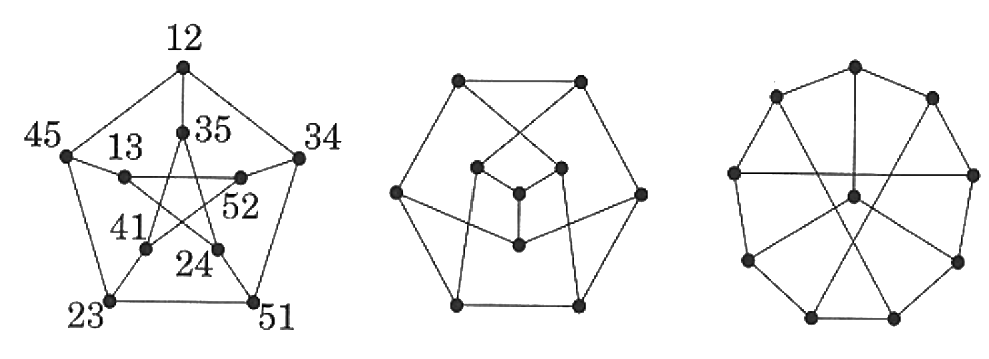
\includegraphics[width=.5\textwidth]{con-petersen-examples}
  \caption{Examples of Petersen graphs.}
  \label{fig:con-petersen-examples}
\end{figure}

\begin{proposition}{}{con-petersen-neighbor}
  (1.1.38. Proposition in text)
  If two vertices are nonadjacent in Petersen graph, then they have exactly one common neighbor.
\end{proposition}

\textbf{Proof} of \cref{prop:con-petersen-neighbor}:

\begin{enumerate*}
  \item Any two nonadjacent vertices share one element, and their union $S$ has 3 elements.
        \begin{enumerate}
          \item For example, the vertices 12 and 23 in the leftmost graph in \cref{fig:con-petersen-examples} share the element 2.
          \item For a simple graph with three vertices and two edges, there are 6 elements chosen from 5 elements for three vertices. As a result, at least one element appears twice in this graph. This is proven by \cref{princ:intro-pigeonhole} (pigeonhole principle).
        \end{enumerate}
  \item A vertex adjacent to two vertices is a 2-set (a set with two elements) disjoint from both its neighbors.
  \item Since the 2-sets are chosen from $\{ 1,\, 2,\, 3,\, 4,\, 5 \}$, there is exactly one 2-set disjoint from $S$ (defined in the first point).
\end{enumerate*}

\begin{corollary}{}{con-petersen-girth}
  (1.1.40. Corollary in text)
  The Petersen graph has girth 5.
\end{corollary}

\textbf{Proof} of \cref{cor:con-petersen-girth}:
\begin{enumerate*}
  \item The graph is simple, for it has no 1-cycle or 2-cycle.
  \item A 3-cycle require three pairwise disjoint 2-sets, which can not occur among 5 elements.
  \item A 4-cycle in the absence of 3-cycles would require nonadjacent vertices with two common neighbors, which violates \cref{prop:con-petersen-neighbor}.
  \item The vertices 12, 34, 51, 23, 45 form a 5-cycle, so the girth is 5.
\end{enumerate*}

In the proof above, it proves \cref{cor:con-petersen-girth} by proving the impossibility of 1-cycle, 2-cycle, 3-cycle and 4-cycles. We don't need to prove cycles with more than 5 vertices because the girth of a graph is defined by the shortest cycle, which is 5 in the Petersen graph.

\subsubsection{Automorphism}

\begin{definition}{}{}
  (1.1.41. Definition in text)
  An \textbf{automorphism} of $G$ is an isomorphism from $G$ to $G$.

  A graph $G$ is \textbf{vertex-transitive} if for every pair $u,\, v \in V(G)$, there is an automorphism that maps $u$ to $v$.
\end{definition}

Automorphism refers to an isomorphism for only one single graph. \supp{By humand eyes, we regard symmetric objects beautiful.} In graph theory, if we make swaps of vertices such that the graph is identical to the original one, we get a automorphism for these swapping.

\begin{wrapfigure}{r}{0.3\textwidth}
  \centering
  \centering
  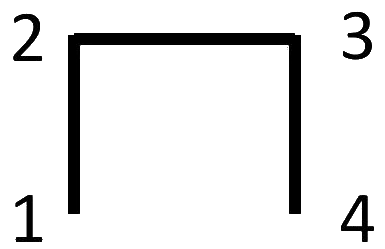
\includegraphics[width=.28\textwidth]{con-automorphism-en}
  \caption{A graph $G$ in N shape.}
  \label{fig:con-automorphism-en}
\end{wrapfigure}

(1.1.42.* Example in text) For example, $G$ as shown in \cref{fig:con-automorphism-en} is the path with $V(G) = \{ 1,\, 2,\, 3,\, 4 \}$ and $E(G) = \{ 12,\, 23,\, 34 \}$. It has two automorphisms: (1) the identity permutation (a vertex swapping with itself) and (2) the permutation $1 \leftrightarrow 4$ and $2 \leftrightarrow 3$ because we could mirror the vertices 1 and 2 to vertices 4 and 3 respectively such that the graph "looks" as the original one without a bijection function.

Question 1: Is it an automorphism if only vertices 1 and 2 are swapped in $G$?\\
Answer: No. Since we need a bijection function to make the swapped graph "look like" the original one, it's not an automorphism; it's an isomorphism.

Question 2: Is $G$ isomorphic to the graph $H$ which is obtained from only swapping vertices 1 and 2 of $G$?\\
Answer: Yes. Please refer to the previous answer.

\begin{wrapfigure}{r}{0.3\textwidth}
  \centering
  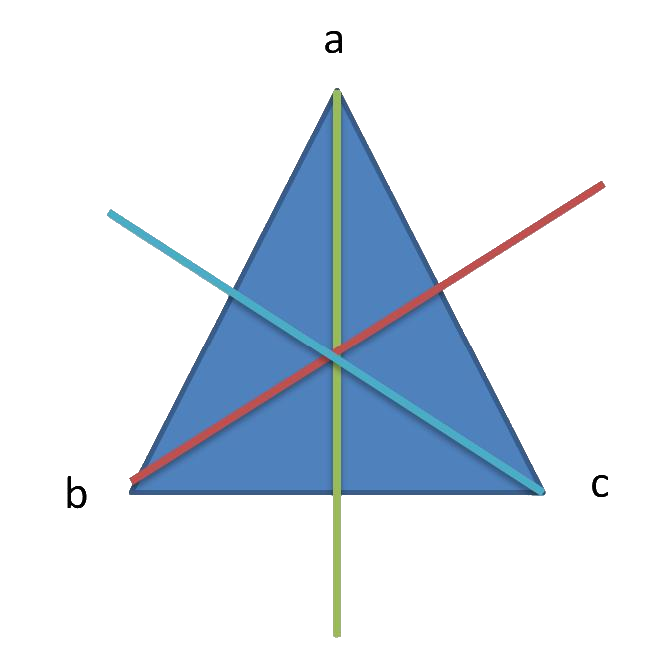
\includegraphics[width=.28\textwidth]{con-automorphism-triangle}
  \caption{A graph $G$ in triangle.}
  \label{fig:con-automorphism-triangle}
\end{wrapfigure}

Given a graph $G$ as shown in \cref{fig:con-automorphism-triangle}, we know that automorphism of $G$ is a permutation function $\func{P}{V(G)}{V(G)}$ such that $P(u)P(v) \in E(G) \iff uv \in E(G)$. That is, the permutation function $P$ preserves adjacency and non-adjacency in graph $G$.

Along the green line passing through the vertex $a$, by mirroring the graph (swapping vertices $b$ and $c$), we have the following mapping of vertices before and after:
\begin{enumerate*}
  \def\mapping#1#2{Old vertex $#1$ $\rightarrow$ new vertex $#2$.}%
  \item \mapping{a}{a}
  \item \mapping{b}{c}
  \item \mapping{c}{b}
\end{enumerate*}

Not only can we mirror a graph, but also we can rotate a graph as follows.

In matrix representation of an automorphism, the first (topmost) row is the vertices before mapping; the last (bottom) row is the mapped ones.

In clause representation (?) of an automorphism, each vertex in a clause (a pair of parentheses) rotates left.

Identity automorphism means vertices are swapped with themselves. Reflection automorphism manes mirroring a graph.

\begin{center}
  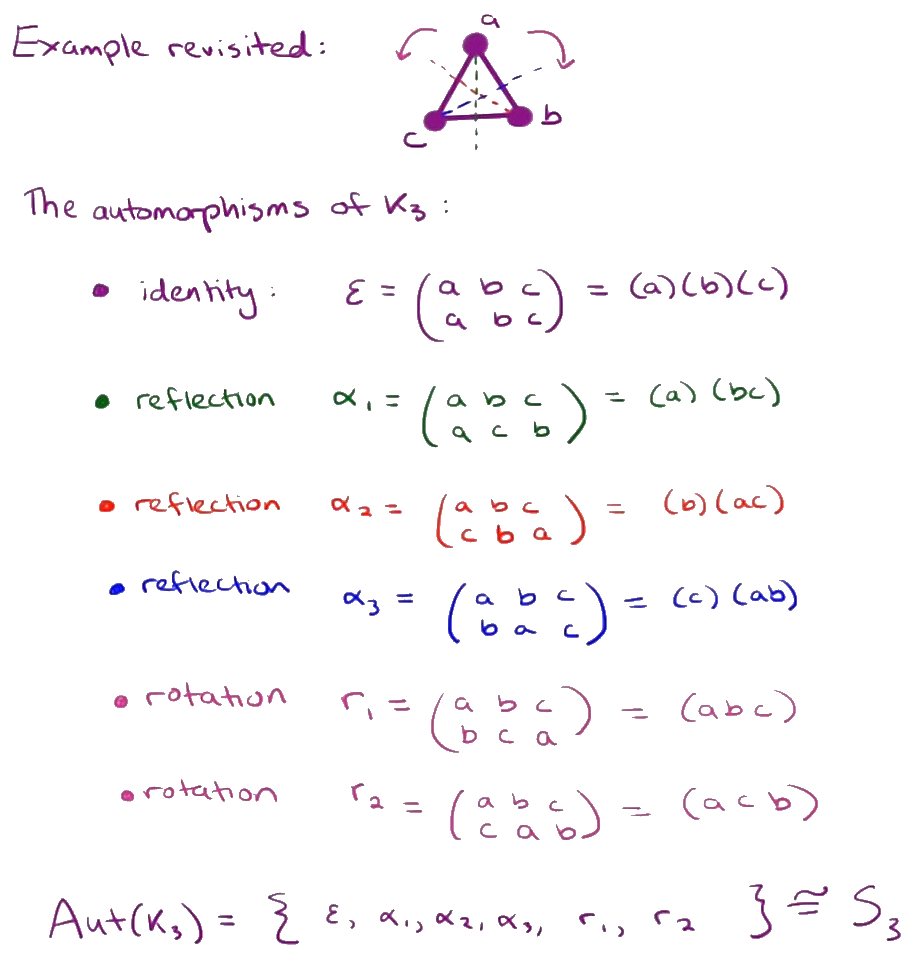
\includegraphics[width=.5\textwidth]{con-automorphism-rotation}
\end{center}

How can you say that a graph is more symmetric than the other one? You need the calculate the number of automorphisms in them.

\begin{center}
  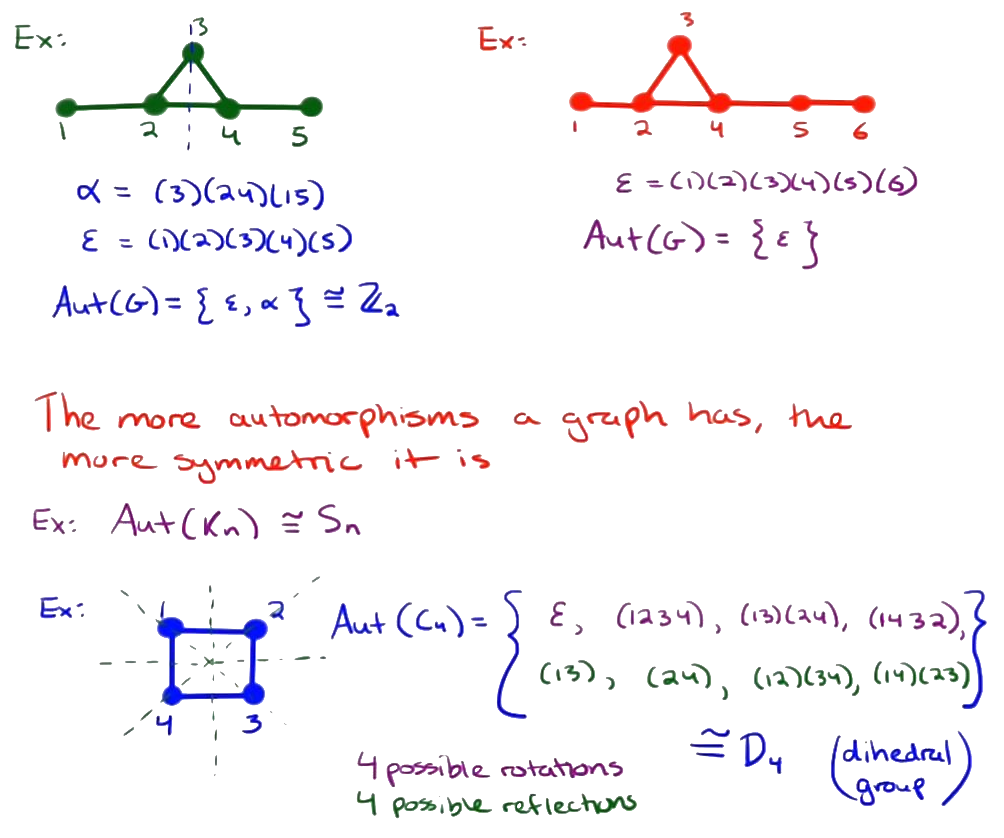
\includegraphics[width=.5\textwidth]{con-automorphism-comparison}
\end{center}
The characteristics of automorphisms are important to some extent.

Reference: Sarada Herke. (2015). "Graph Theory FAQs: 02. Graph Automorphisms" on YouTube. [Online]. \url{https://www.youtube.com/watch?v=X4_4Bqj6EdA}. Accessed on 2024-03-28.

\subsubsection{Paths, Cycles and Trails}

\begin{definition}{}{con-walk-trail}
  (1.2.2. Definition in text)
  A \textbf{walk} is a list $v_0,\, e_1,\, v_1,\, \ldots,\, e_k,\, v_k$ of vertices and edges, such that for $1 \leq i \leq k$, the edges $e_i$ has endpoints $v_{i-1}$ and $v_i$.

  A \textbf{trail} is a walk with \textbf{no repeated edge}.
\end{definition}

In a walk or trail, there could be repeated vertices.

For example, recall the seven bridge problem in \cref{subsubsec:con-seven-bridges}. The list $W_1$ below is a closed walk of length 5 rather than a trail. The list $T_1$ below is a trail.

\begin{align*}
  W_1 = x,\, e_2,\, w,\, e_5,\, y,\, e_6,\, x,\, e_1,\, w,\, e_2,\, x \\
  T_1 = x,\, e_2,\, w,\, e_5,\, y,\, e_6,\, x,\, e_1,\, w
\end{align*}

% TODO FIXME: modify \reusablefigure to receive subfigure
\begin{figure}[ht]
  \centering
  \begin{subfigure}{0.35\textwidth}
    \centering
    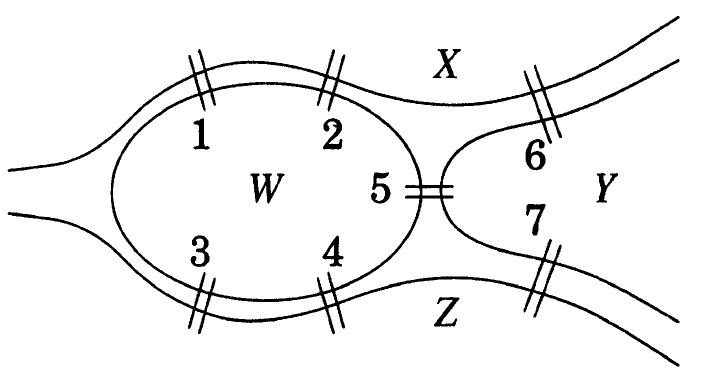
\includegraphics[width=\textwidth]{con-seven-bridge-original}
    \caption{Original version.}
  \end{subfigure}
  \hfil
  \begin{subfigure}{0.25\textwidth}
    \centering
    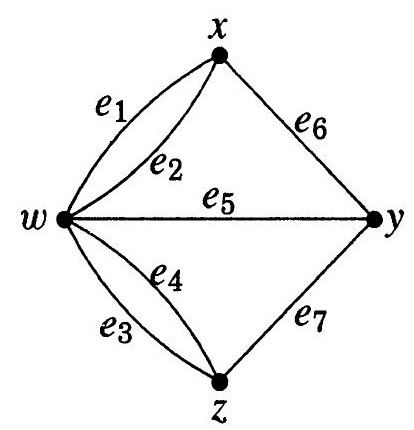
\includegraphics[width=\textwidth]{con-seven-bridge-graph}
    \caption{Graph version.}
  \end{subfigure}
  \caption{Seven-bridge problem.}
\end{figure}

\begin{definition}{}{con-walk-trail-path-endpoints}
  (1.2.2. Definition in text)
  A \textbf{$\bm{u,v}$-walk} or \textbf{$\bm{u,v}$-trail} has first vertex $u$ and last vertex $v$ as its endpoints.
  (A walk or a trail records vertices and edges especially in a multigraph.)

  A \textbf{$\bm{u,v}$-path} is a path whose vertices of degree 1 are $u$ and $v$; the others are \textbf{internal vertices} (usually of degree 2). (A path only records vertices.)

  The \textbf{length} of a walk, trail, path or cycle is the \textbf{number of edges}. (In the length of a path is the number of its vertices minus one.)

  A wal or trail is \textbf{closed} if its endpoints are the same.
\end{definition}

In brief, a $u,v$-path refers to a way to traverse some vertices from $u$ to $v$ via some edges.

See \cref{def:con-path-cycle} for the definition of paths and cycles.

\begin{figure}[htbp]
  \centering
  \begin{subfigure}[t]{.4\textwidth}
    \centering
    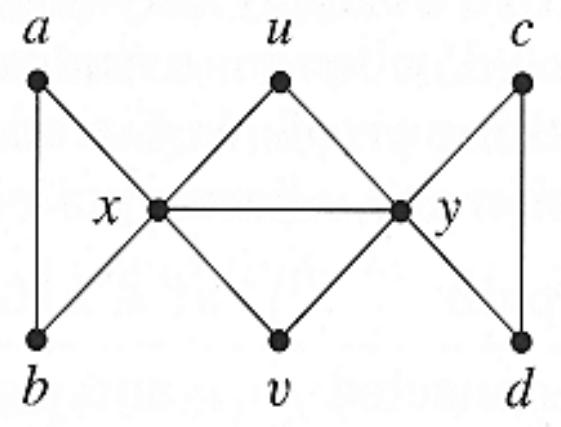
\includegraphics[width=.8\textwidth]{con-walk-original}
    \caption{The original graph with nothing drawn.}
    \label{fig:con-walk-original}
  \end{subfigure}
  \hspace{.1\textwidth}
  \begin{subfigure}[t]{.4\textwidth}
    \centering
    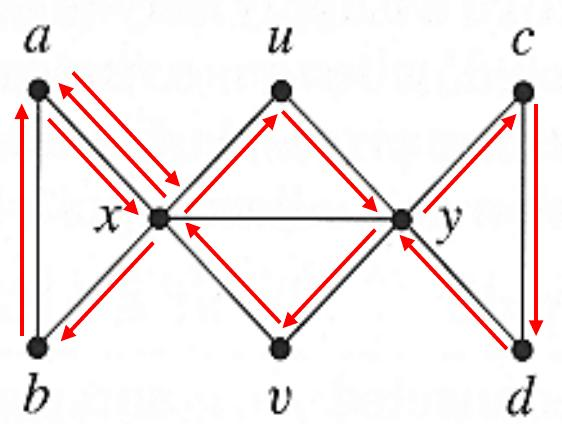
\includegraphics[width=.8\textwidth]{con-walk-closed}
    \caption{A closed $a,a$-walk or an $a,a$-cycle.}
    \label{fig:con-walk-closed}
  \end{subfigure}

  \vspace{2em}

  \begin{subfigure}[t]{.4\textwidth}
    \centering
    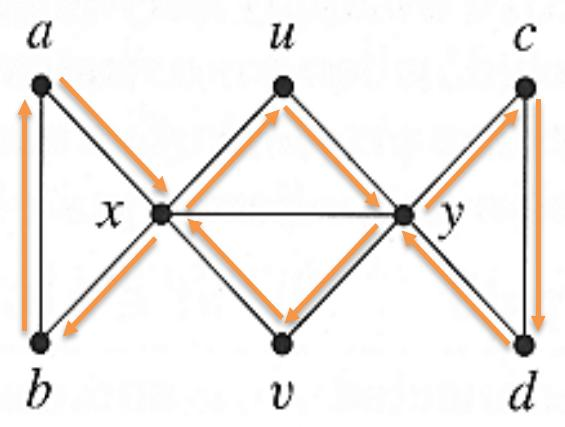
\includegraphics[width=.8\textwidth]{con-trail-closed}
    \caption{A closed $a,a$-trail or an $a,a$-cycle.}
    \label{fig:con-trail-closed}
  \end{subfigure}
  \hspace{.1\textwidth}
  \begin{subfigure}[t]{.4\textwidth}
    \centering
    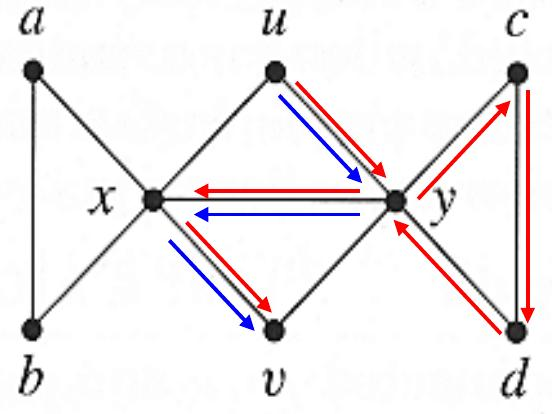
\includegraphics[width=.8\textwidth]{con-trail-path}
    \caption{A $u,v$-trail $u,\, y,\, c,\, d,\, y,\, x,\, v$ contains $u,v$-path $u,\, y,\, x,\, v$ but not $u,\, y,\, v$.}
    \label{fig:con-trail-path}
  \end{subfigure}

  \vspace{2em}

  \begin{subfigure}[t]{.4\textwidth}
    \centering
    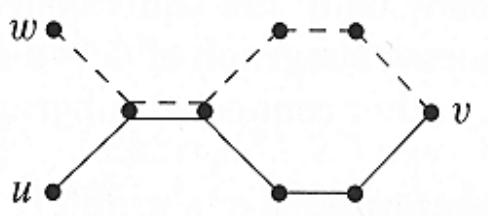
\includegraphics[width=.8\textwidth]{con-walk-path-example}
    \caption{A $u,v$-walk contains a $u,w$-path. See \cref{lem:con-walk-path} and its proof.}
    \label{fig:con-walk-path-example}
  \end{subfigure}
  \hspace{.1\textwidth}
  \begin{subfigure}[t]{.4\textwidth}
    \centering
    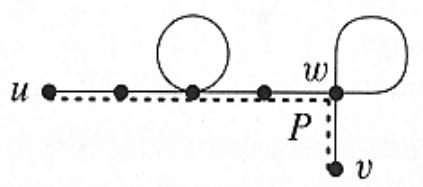
\includegraphics[width=.8\textwidth]{con-walk-path-proof}
    \caption{A graph for the illustration of the proof of \cref{lem:con-walk-path}.}
    \label{fig:con-walk-path-proof}
  \end{subfigure}

  \caption{Illustrations for walks and trails.}
  \label{fig:con-walk-trail}
\end{figure}

\begin{theorem}{String Principle of Induction}{con-strong-induction}
  (1.2.1. Theorem in text)
  Let $P(n)$ be a statement with an integer parameter $n$.
  If the following two conditions hold, then $P(n)$ is true for each positive integer $n$.

  \begin{enumerate*}
    \item P(1) is true.
    \item For all $n > 1$, "$P(k)$ is true for $1 \leq k < n$" implies "$P(n)$ is true".
  \end{enumerate*}
\end{theorem}

Continuing from \cref{thm:con-strong-induction}, if you cannot show that "all" cases from the base case $P(1)$ to $P(n-1)$ true, you cannot use strong principle of induction to say $P(n)$ true.

In strong principle of induction in \cref{thm:con-strong-induction} we prove $P(n)$ true under $P(1)$ to $P(n - 1)$ true, rather than proving $P(n + 1)$ true under $P(1)$ to $P(n)$ true as we do in principle of induction in \cref{princ:intro-induction}.

\begin{lemma}{}{con-walk-path}
  (1.2.5. Lemma in text)
  Every $u,v$-walk contains a $u,v$-path.
\end{lemma}

Note that proof of a theorem (lemma, principle, $\ldots$) must be applicable for all graphs in the domain instead of some limited cases. And you couldn't assume $P(n - 1)$ true without a proof because $P(n - 1)$ may be false.

\textbf{Proof} of \cref{lem:con-walk-path} using strong principle of induction in \cref{thm:con-strong-induction}:
By induction for a $u,v$-walk $W$ whose length is $l$ as illustrated in \cref{fig:con-walk-path-proof}:
\begin{enumerate*}
  \item Basis step: When $l = 0$, $W$ contains a single vertex as a path whose length is 0.
  \item Induction step: When $l \geq 1$, there are two possible cases as follows.
        \begin{enumerate}
          \item Case 1: $W$ has no repeated vertex, so $W$ is a $u,v$-path (if we see only the sequence of vertices in $W$).
          \item Case 2: $W$ has a repeated vertex $w$. (This case covers all cases with any positive number of repeated vertices.) Thus, there is a $u,u$-loop or $u,u$-cycle. By removing that loop or cycle, we get a $u,v$-path.
        \end{enumerate}
\end{enumerate*}

\begin{definition}{}{con-connected-path}
  (1.2.6. Definition in text)
  A graph $G$ is \textbf{connected} if it has a $u,v$-path whenever $u,v \in V(G)$; otherwise, $G$ is \textbf{disconnected}.

  If $G$ has a $u,v$-path, then $u$ is \textbf{connected} to $v$ in $G$.

  The \textbf{connection relation} on $V(G)$ consists of the \textbf{ordered pairs} $(u,\, v)$ such that $u$ is connected to $v$. (In our primary textbook, $uv$ refers to an edge between $u$ and $v$ while $(u,\, v)$ may not imply an edge $uv$. Also note that $(u,\, v)$ and $(v,\, u)$ refer to two paths.)
\end{definition}

\begin{wrapfigure}{r}{.3\textwidth}
  \centering
  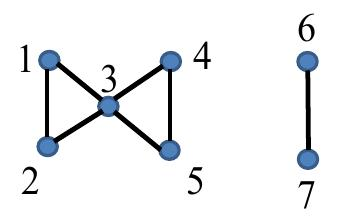
\includegraphics[width=.28\textwidth]{con-connected-path}
  \caption{A graph $G$ for the illustration of connection relation.}
  \label{fig:con-connected-path}
\end{wrapfigure}

Connection relation in \cref{def:con-connected-path} is an equivalence relation defined in \cref{def:intro-equiv-relation}. That is, it satisfies reflexive, symmetric and transitive properties. A path from $u$ to itself satisfies the reflexive property; in an undirected graph, a path from $u$ to $v$ implies a path from $v$ to $u$; $(v_1,\, v_2)$ and $(v_2,\, v_3)$ imply $(v_1,\, v_3)$.

Question 1: Is the graph $G$ in \cref{fig:con-connected-path} connected? List all equivalence classes.\\
Answer: There are two equivalence classes, $\{1,\, 2,\, 3,\, 4,\, 5\}$ and $\{6,\, 7\}$, so this graph is not connected. These two equivalence classes also form two connected components.

Question 2: How to write the connection relation on $V(G)$ in \cref{fig:con-connected-path}?\\
Answer: $\{ 1,\, 2,\, 3,\, 4,\, 5 \}^2, \{ 6,\, 7 \}^2$. (Please refer to the cartesian product defined in \cref{rem:intro-tuple-ordered-pair}.)

\begin{definition}{}{con-component}
  (1.2.8. Definition in text)
  The \textbf{connected components} or \textbf{components} of a graph $G$ are its (locally) \textbf{maximal} connected subgraphs.
\end{definition}

\subsection{Vertex Degrees and Counting}

% TODO: p.35

\subsection{Directed Graphs}

\end{document}